\documentclass{article}
\usepackage[utf8]{inputenc}
\usepackage[brazil]{babel}
\usepackage[a4paper, top=2.5cm, bottom=2.5cm, left=2cm, right=2.5cm]{geometry}
\usepackage{makecell}

\usepackage{hyperref}

\usepackage{amsmath,amssymb}
\newcommand*{\RandomVariable}[1]{\mathbf{#1}}
\newcommand*{\ExpectedValue}{\mathbb{E}}

\usepackage{graphicx}
\graphicspath{{figures/}}
\usepackage{subcaption}

\usepackage{pgf}
\usepackage{tikz}
\usetikzlibrary{arrows,automata,plotmarks}
\usepackage{pgfplots}
\pgfplotsset{compat=1.15}

\tikzset{
    % node styles
    state-node/.style={
        fill=none, shape=circle, draw=black, thick, text=black, minimum size=0.6cm},
    action-node/.style={
        fill=black, draw=none, text=white, shape=circle, inner sep=0.05cm, minimum size=0.2cm},
    reward-node/.style={
        fill=none, draw=black, text=black},
    hidden-node/.style={
        fill=none, draw=none, text=white, shape=circle, inner sep=0,outer sep=0, minimum size=0.0cm},
    % label styles
    action-label/.style={
        shape=circle, text=white, draw=none, fill=black, inner sep=0.05cm, minimum size=0.2cm, align=center, yshift=0.0cm, anchor=center},
    reward-label/.style={
        shape=rectangle, text=black, draw=black, fill=white, minimum size=0.5cm, align=center, yshift=0.0cm, anchor=center},
    hidden-edge/.style={
        text=white, draw=none, fill=none, inner sep=0,outer sep=0, minimum size=0.0cm},
}


% Diagrama de interação
\newcommand{\rlinteraction}{
    \begin{tikzpicture}[->,>=latex, auto, node distance=2.0cm, very thick, font=\small]
        \tikzstyle{rect-node}=[fill=none,shape=rectangle,draw=black,text=black,rounded corners=0.1cm, inner sep=0.4cm]
        \tikzstyle{hidden-node}=[fill=none, draw=none, text=black, shape=rectangle, inner sep=0,outer sep=0.05cm, minimum height=0.75cm]
        
        \node[rect-node]  (Agent)                                     {\normalsize Agent};
        \node[rect-node]  (Env)     [below of=Agent]                  {\normalsize Environment};
        \node[hidden-node] (Hidden)  [left of=Env, xshift=-0.5cm]     {};
        \node[hidden-node] (UpHid)   [above of=Hidden, yshift=-1.0cm] {};
        \node[hidden-node] (DownHid) [below of=Hidden, yshift=1.0cm]  {};
        
        \draw[thick, transform canvas={yshift=0.25cm}] (Env) to node[above] 
            {$R_{t+1}$} (Hidden);
        \draw[ultra thick, transform canvas={yshift=-0.25cm}] (Env) to node[above] 
            {$S_{t+1}$} (Hidden);
        \draw[ultra thick] (Hidden.255) to node[left, pos=1.0, yshift=1.25cm, align=center] 
            {state\\$S_t$}  ++(-1.5,0) |- (Agent.165);
        \draw[thick] (Hidden.105) to node[right, pos=1.0, yshift=0.75cm, align=center] 
            {reward\\$R_t$} ++(-1.0,0) |- (Agent.195);
        \draw[ultra thick] (Agent) to node[below right, pos=1.0, yshift=-0.5cm, align=center] 
            {action\\$A_t$} ++(3.5,0)  |- (Env);
        \draw[-, thick, dashed] (UpHid) to node {} (DownHid);
    \end{tikzpicture}
}


\newcommand{\rlinteractionpomdp}{
    \begin{tikzpicture}[->,>=latex, auto, node distance=2.0cm, very thick, font=\small]
        \tikzstyle{rect-node}=[fill=none,shape=rectangle,draw=black,text=black,rounded corners=0.1cm, inner sep=0.4cm]
        \tikzstyle{hidden-node}=[fill=none, draw=none, text=black, shape=rectangle, inner sep=0,outer sep=0.05cm, minimum height=0.75cm]
        
        \node[rect-node] (Agent) {\normalsize Agent};
        \node[rect-node] (Env) [right of=Agent, xshift=4.0cm] {\normalsize Environment};
        \node[hidden-node] (Hidden) [below of=Env, xshift=-2.0cm, yshift=0.5cm] {};
        \node[hidden-node] (UpHid) [above of=Hidden, yshift=-1.0cm] {};
        \node[hidden-node] (DownHid) [below of=Hidden, yshift=1.0cm] {};
        \node[hidden-node] (Reward) [below of=Env, xshift=0.25cm, yshift=0.5cm] {};
        
        \draw[thick, transform canvas={yshift=-0.25cm}] (Reward) to node[below, yshift=-0.1cm] 
            {$R_{t+1}$} (Hidden);
            
        \draw[ultra thick, transform canvas={xshift=0.10cm}] (Env.260) to node[xshift=-0.5cm, yshift=-0.4cm] {$O_{t+1}$} ++(0,0) |- (Hidden.105);
            
        \draw[ultra thick] (Hidden.105) to node[above, xshift=-1.5cm, align=center] 
            {observation\\$O_t$}  ++(0,0) -| (Agent.290);
        \draw[thick] (Hidden.255) to node[below, xshift=-1.5cm, align=center] 
            {reward\\$R_t$} ++(0,0) -| (Agent.250);
            
        \draw[ultra thick] (Agent) to node[xshift=3.5cm, align=center] 
            {action\\$A_t$} ++(0,1.5) -| (Env);
            
        \draw[-, thick, dashed] (UpHid) to node {} (DownHid);
    \end{tikzpicture}
}


\newcommand{\mdpthreestate}{
    \begin{tikzpicture}[->,>=stealth', auto, node distance=4.0cm, thick]
        \node[state-node]  (S1) {$s_1$};
        \node[state-node]  (S2) [below of=S1, xshift=-3.0cm] {$s_2$};
        \node[state-node]  (S3) [below of=S1, xshift= 3.0cm] {$s_3$};
        \node[action-node] (A1) [below of=S1, yshift=2.5cm, xshift=-3.0cm] {$a_1$};
        \node[action-node] (A2) [below of=S1, yshift=2.5cm]  {$a_2$};
        \node[action-node] (A3) [below of=S1, yshift=2.5cm, xshift=2.6cm] {$a_3$};
        
        \draw[bend right=20,-] (S1) to node[]  {} (A1);
        \draw[-]               (S1) to node[]  {} (A2);
        \draw[bend left=20,-] (S1) to node[]  {} (A3);
        
        \draw[bend right=30]   (A1) to node[left, pos=0.2]  {$p_1$} (S2);
        \draw[bend left=30]    (A1) to node[right, pos=0.2] {$p_2$} (S2);
        \draw[bend left=40]    (A2) to node[left, pos=0.3]  {$p_3$} (S2);
        \draw[bend right=40]   (A2) to node[right, pos=0.3] {$p_4$} (S3);
        \draw[bend left=20]    (A3) to node[right, pos=0.2] {$1$} (S3);
        
        \draw[hidden-edge, bend right=30] (A1) to node[reward-label] {$r_1$} (S2);
        \draw[hidden-edge, bend left=30]  (A1) to node[reward-label] {$r_2$} (S2);
        \draw[hidden-edge, bend left=40]  (A2) to node[reward-label] {$r_3$} (S2);
        \draw[hidden-edge, bend right=40] (A2) to node[reward-label] {$r_4$} (S3);
        \draw[hidden-edge, bend left=20]  (A3) to node[reward-label] {$r_5$} (S3);
    \end{tikzpicture}
}

\newcommand{\mdpthreestatenoprobs}{
    \begin{tikzpicture}[->,>=stealth', auto, node distance=4.0cm, thick]
        \node[state-node]  (S1) {$s_1$};
        \node[state-node]  (S2) [below of=S1, xshift=-3.0cm] {$s_2$};
        \node[state-node]  (S3) [below of=S1, xshift= 3.0cm] {$s_3$};
        \node[action-node] (A1) [below of=S1, yshift=2.5cm, xshift=-3.0cm] {$a_1$};
        \node[action-node] (A2) [below of=S1, yshift=2.5cm]  {$a_2$};
        \node[action-node] (A3) [below of=S1, yshift=2.5cm, xshift=2.6cm] {$a_3$};
        
        \draw[bend right=20,-] (S1) to node[]  {} (A1);
        \draw[-]               (S1) to node[]  {} (A2);
        \draw[bend left=20,-] (S1) to node[]  {} (A3);
        
        \draw[bend right=30] (A1) to node[reward-label] {$r_1$} (S2);
        \draw[bend left=30]  (A1) to node[reward-label] {$r_2$} (S2);
        \draw[bend left=40]  (A2) to node[reward-label] {$r_3$} (S2);
        \draw[bend right=40] (A2) to node[reward-label] {$r_4$} (S3);
        \draw[bend left=20]  (A3) to node[reward-label] {$r_5$} (S3);
    \end{tikzpicture}
}

\newcommand{\mdpbig}{
    \begin{tikzpicture}[->,>=stealth',auto,node distance=3.5cm, thick]
        \node[state-node] (S1)                     {$s_1$};
        \node[state-node] (S2) [above right of=S1] {$s_2$};
        \node[state-node] (S3) [below right of=S1, xshift=1.0cm] {$s_3$};
        \node[state-node] (S4) [below right of=S2] {$s_4$};
        \node[state-node] (S5) [right of=S4, xshift=-1.0cm]       {$s_5$};
        
        \node[action-node] (A1) [right of=S1, xshift=-2.0cm, yshift=0.5cm] {$a_1$};
        \node[action-node] (A3) [left of=S3, xshift=1.5cm, yshift=1.0cm] {$a_3$};
        \node[action-node] (A4) [below of=S4, xshift=0.75cm, yshift=2.0cm] {$a_4$};
        
        % from (S1)
        \draw[-] (S1) to node[] {} (A1);
        \draw[bend right=20] (A1) to node[left, pos=0.25] {$p_1$} (S2);
        \draw[bend left=20] (A1) to node[below, pos=0.25] {$p_2$} (S4);
        \draw[hidden-edge, bend right=20] (A1) to node[reward-label, pos=0.55] {$r_1$} (S2);
        \draw[hidden-edge, bend left=20] (A1) to node[reward-label, pos=0.60] {$r_2$} (S4);
        
        % from (S2)
        \draw[bend left=20] (S2) to node[action-label, pos=0.25] {$a_2$} (S4);
        \draw[hidden-edge, bend left=20] (S2) to node[reward-label, pos=0.65] {$r_3$} (S4);
        
        % from (S3)
        \draw[-, bend right=50] (S3) to node[] {} (A3);
        \draw[bend left=40] (A3) to node[above, pos=0.2] {$p_3$} (S1);
        \draw[bend right=40] (A3) to node[left, pos=0.3] {$p_4$} (S3);
        \draw[hidden-edge, bend left=40] (A3) to node[reward-label, pos=0.6] {$r_4$} (S1);
        \draw[hidden-edge, bend right=40] (A3) to node[reward-label, pos=0.6] {$r_5$} (S3);
        
        % from (S4)
        \draw[-] (S4) to node[] {} (A4);
        \draw[bend left=40] (A4) to node[left, pos=0.2] {$p_3$} (S3);
        \draw[bend right=40] (A4) to node[above, pos=0.25] {$p_4$} (S5);
        \draw[hidden-edge, bend left=40] (A4) to node[reward-label, left, pos=0.55] {$r_6$} (S3);
        \draw[hidden-edge, bend right=40] (A4) to node[reward-label, above right, pos=0.5] {$r_7$} (S5);
        
        % from (S5)
        \draw[bend right] (S5) to node[action-label, pos=0.25] {$a_5$} (S2);
        \draw[hidden-edge, bend right] (S5) to node[reward-label, pos=0.65] {$r_8$} (S2);
        
    \end{tikzpicture}
}


\newcommand{\simplebandit}{
    \begin{tikzpicture}[-,>=stealth', auto, node distance=1.5cm, thick]
        \node[state-node]  (SimpleBanditS1) {$s$};
        \node[reward-node] (SimpleBanditR1) [below of=SimpleBanditS1, xshift=-1.0cm] {$r$};
        \node[reward-node] (SimpleBanditR2) [below of=SimpleBanditS1, xshift=0.0cm]  {$r$};
        \node[reward-node] (SimpleBanditR3) [below of=SimpleBanditS1, xshift=1.0cm]  {$r$};
        
        \draw[bend right] (SimpleBanditS1) to node[action-label] {$a$} (SimpleBanditR1);
        \draw             (SimpleBanditS1) to node[action-label] {$a$} (SimpleBanditR2);
        \draw[bend left]  (SimpleBanditS1) to node[action-label] {$a$} (SimpleBanditR3);
    \end{tikzpicture}
}

\newcommand{\associativebandits}{
    \begin{tikzpicture}[thick]
        \node[draw=black] (AB1) {
            \begin{tikzpicture}[]
                \node[] (B1) {
                    \simplebandit
                };
                \node[right of=B1, xshift=2.0cm] (B2) {
                    \simplebandit
                };
                \node[right of=B2, xshift=2.0cm] (B3) {
                    \simplebandit
                };
                \node[right of=B3, xshift=1.0cm] (B4) {
                    $\boldsymbol{\cdots}$
                };
                \node[right of=B4, xshift=1.0cm] (B5) {
                    \simplebandit
                };
            \end{tikzpicture}
        };
        
        \node[draw=black, below of=AB1, yshift=-2.0cm] (AB2) {
            \begin{tikzpicture}[]
                \node[] (B1) {
                    \simplebandit
                };
                \node[right of=B1, xshift=2.0cm] (B2) {
                    \simplebandit
                };
                \node[right of=B2, xshift=2.0cm] (B3) {
                    \simplebandit
                };
                \node[right of=B3, xshift=1.0cm] (B4) {
                    $\boldsymbol{\cdots}$
                };
                \node[right of=B4, xshift=1.0cm] (B5) {
                    \simplebandit
                };
            \end{tikzpicture}
        };
        
        \node[below of=AB2, yshift=-1.0cm] (AB3) {
            $\Huge\vdots$
        };
    
        \node[draw=black, below of=AB3, yshift=-1.0cm] (AB4) {
            \begin{tikzpicture}[]
                \node[] (B1) {
                    \simplebandit
                };
                \node[right of=B1, xshift=2.0cm] (B2) {
                    \simplebandit
                };
                \node[right of=B2, xshift=2.0cm] (B3) {
                    \simplebandit
                };
                \node[right of=B3, xshift=1.0cm] (B4) {
                    $\boldsymbol{\cdots}$
                };
                \node[right of=B4, xshift=1.0cm] (B5) {
                    \simplebandit
                };
            \end{tikzpicture}
        };
        
        \draw[->, thick] (AB1) to node {} (AB2);
        \draw[->, thick] (AB2) to node {} (AB3);
        \draw[->, thick] (AB3) to node {} (AB4);
    \end{tikzpicture}
}

\newcommand{\fullrldiagram}{
    \begin{tikzpicture}[-,>=stealth', auto, node distance=1.5cm, thick]
        \node[state-node] (S1) {$s$};
        \node[reward-node] (R1S1) [below of=S1, xshift=-1.0cm] {$r$};
        \node[reward-node] (R2S1) [below of=S1]                {$r$};
        \node[reward-node] (R3S1) [below of=S1, xshift=1.0cm]  {$r$};
        
        \draw[bend right] (S1) to node[action-label] {$a$} (R1S1);
        \draw[]           (S1) to node[action-label] {$a$} (R2S1);
        \draw[bend left]  (S1) to node[action-label] {$a$} (R3S1);
        
        \node[state-node] (S2) [right of=S1, xshift=2.0cm] {$s$};
        \node[reward-node] (R1S2) [below of=S2, xshift=-1.0cm] {$r$};
        \node[reward-node] (R2S2) [below of=S2]                {$r$};
        \node[reward-node] (R3S2) [below of=S2, xshift=1.0cm]  {$r$};
        
        \draw[bend right] (S2) to node[action-label] {$a$} (R1S2);
        \draw[]           (S2) to node[action-label] {$a$} (R2S2);
        \draw[bend left]  (S2) to node[action-label] {$a$} (R3S2);
        
        \node[right of=S2, xshift=0.65cm, yshift=-0.75cm] (DOTS1) {
            $\boldsymbol{\cdots}$
        };
        
        \node[state-node] (S3) [right of=S2, xshift=3.0cm] {$s$};
        \node[reward-node] (R1S3) [below of=S3, xshift=-1.0cm] {$r$};
        \node[reward-node] (R2S3) [below of=S3]                {$r$};
        \node[reward-node] (R3S3) [below of=S3, xshift=1.0cm]  {$r$};
        
        \draw[bend right] (S3) to node[action-label] {$a$} (R1S3);
        \draw[]           (S3) to node[action-label] {$a$} (R2S3);
        \draw[bend left]  (S3) to node[action-label] {$a$} (R3S3);
        
        
        \node[state-node] (S4) [below of=S1, yshift=-2.0cm] {$s$};
        \node[reward-node] (R1S4) [below of=S4, xshift=-1.0cm] {$r$};
        \node[reward-node] (R2S4) [below of=S4]                {$r$};
        \node[reward-node] (R3S4) [below of=S4, xshift=1.0cm]  {$r$};
        
        \draw[bend right] (S4) to node[action-label] {$a$} (R1S4);
        \draw[]           (S4) to node[action-label] {$a$} (R2S4);
        \draw[bend left]  (S4) to node[action-label] {$a$} (R3S4);
        
        \node[state-node] (S5) [right of=S4, xshift=2.0cm] {$s$};
        \node[reward-node] (R1S5) [below of=S5, xshift=-1.0cm] {$r$};
        \node[reward-node] (R2S5) [below of=S5]                {$r$};
        \node[reward-node] (R3S5) [below of=S5, xshift=1.0cm]  {$r$};
        
        \draw[bend right] (S5) to node[action-label] {$a$} (R1S5);
        \draw[]           (S5) to node[action-label] {$a$} (R2S5);
        \draw[bend left]  (S5) to node[action-label] {$a$} (R3S5);
        
        \node[right of=S5, xshift=0.65cm, yshift=-0.75cm] (DOTS2) {$\boldsymbol{\cdots}$};
        
        \node[state-node] (S6) [right of=S5, xshift=3.0cm] {$s$};
        \node[reward-node] (R1S6) [below of=S6, xshift=-1.0cm] {$r$};
        \node[reward-node] (R2S6) [below of=S6]                {$r$};
        \node[reward-node] (R3S6) [below of=S6, xshift=1.0cm]  {$r$};
        
        \draw[bend right] (S6) to node[action-label] {$a$} (R1S6);
        \draw[]           (S6) to node[action-label] {$a$} (R2S6);
        \draw[bend left]  (S6) to node[action-label] {$a$} (R3S6);
        
        
        \draw[->, out=-90, in=90] (R1S1) to node[] {} (S5);
        \draw[->, out=-90, in=90] (R2S1) to node[] {} (S6);
        \draw[->, out=-90, in=90] (R3S1) to node[] {} (S4);
        
        \draw[->, out=-90, in=90] (R1S2) to node[] {} (DOTS2);
        \draw[->, out=-90, in=90] (R2S2) to node[] {} (S4);
        \draw[->, out=-90, in=90] (R3S2) to node[] {} (S5);
        
        \draw[->, out=-90, in=90] (R1S3) to node[] {} (S6);
        \draw[->, out=-90, in=90] (R2S3) to node[] {} (DOTS2);
        \draw[->, out=-90, in=90] (R3S3) to node[] {} (DOTS2);
        
        
        \node[below of=S4, yshift=-2.0cm] (DOTS3) {$\Huge\vdots$};
        \node[right of=DOTS3, xshift=2.0cm] (DOTS4) {$\Huge\vdots$};
        \node[right of=DOTS4, xshift=0.65cm] (DOTS5) {$\boldsymbol{\cdots}$};
        \node[right of=DOTS4, xshift=3.0cm] (DOTS6) {$\Huge\vdots$};
        
        
        \draw[->, out=-90, in=90] (R1S4) to node[] {} (DOTS4);
        \draw[->, out=-90, in=90] (R2S4) to node[] {} (DOTS3);
        \draw[->, out=-90, in=90] (R3S4) to node[] {} (DOTS5);
        
        \draw[->, out=-90, in=90] (R1S5) to node[] {} (DOTS5);
        \draw[->, out=-90, in=90] (R2S5) to node[] {} (DOTS3);
        \draw[->, out=-90, in=90] (R3S5) to node[] {} (DOTS6);
        
        \draw[->, out=-90, in=90] (R1S6) to node[] {} (DOTS4);
        \draw[->, out=-90, in=90] (R2S6) to node[] {} (DOTS4);
        \draw[->, out=-90, in=90] (R3S6) to node[] {} (DOTS5);
    \end{tikzpicture}
}

\newcommand{\todo}[1]{ --\textcolor{red}{\textbf{#1}}--}
%\newcommand{\todo}[1]{}

% PB: redefinir maketitle
\makeatletter
\def\@maketitle
{
    \begin{flushleft}
        \let \footnote \thanks
        {\Large \textbf{\@title} \par}
        \vskip 1em
        {\large \textbf{\@author} \par}
        \vskip 1em
        {\large \textit{\@date}}
    \end{flushleft}
    \par
    \vskip 1.5em
}
\makeatother


\title{Notas de estudo - Aprendizado por Reforço}
\author{Parte 01 - Introdução ao Aprendizado por Reforço}
\date{Paulo Bruno de Sousa Serafim - Out/19 - Fev/20}


\begin{document}

\maketitle

    \section{Avisos}
    
        \subsection{Bibliografia}
        
            Antes de qualquer coisa, fica o aviso: esses estudos foram quase totalmente baseados no livro de introdução ao aprendizado por reforço:
        
            \begin{center}
            \noindent\fbox{%
                \parbox{40em}{%
                    Richard S. Sutton and Andrew G. Barto. \textbf{Reinforcement Learning: An Introduction}. 2nd Edition. MIT Press, Cambridge, MA, 2018.
                }%
            }%
            \end{center}
            
            Naturalmente que consultei outras referências eventualmente, mas, no geral, essas notas são notas de estudo desse livro. Sugiro \textbf{muito fortemente} a leitura dele, principalmente por ser gratuito.
            
            Mais ainda, por considerá-lo como uma fonte básica, não o cito explicitamente ao longo das notas, mas considere que ele é citado implicitamente em todas elas. Portanto, caso queira usar algum trecho encontrado aqui, na maioria dos casos, cite o livro e não as notas.
            
        \subsection{Rigor matemático}
        
            Reforçando: essas notas foram feitas com o objetivo de estudos pessoais. Eu tentei escrevê-las em uma linguagem mais acessível para mim e posso ter sido descuidado em alguns momentos com certos termos.
            
            Dito isso, não tento garantir um rigor matemático em nenhuma das notas. Por exemplo, algumas vezes posso mencionar que tal coisa foi provada como verdade e não pôr a prova ou sequer uma referência a ela.
            
            Outra questão relacionada é a notação utilizada. Utilizo uma notação semelhante à do livro base, mas não exatamente igual. Apesar disso, tento manter a consistência ao longo de todas as notas. Caso ocorram diferenças de notação muito provavelmente foi um equívoco meu e agradeço muito a quem apontá-las.
            
        \subsection{Comunicação, sugestões e críticas}
            
            Ficarei \textbf{muito} agradecido em receber qualquer feedback, em especial sugestões de melhoria, correção de erros e críticas de modo geral. Peço, por gentileza, que se você tiver alguma coisa para dizer, crie uma \emph{issue} no github das notas:
            
            \begin{center}
                \url{https://github.com/paulobruno/RLStudyNotes}
            \end{center}
            
            Caso isso não seja possível para você, pode me contatar da forma como for mais conveniente: linkedin, e-mail e até telefone, se souber.
            
    \section{O que é ``reforço''?}
    
        Antes de começar os estudos de Aprendizado por Reforço, vamos primeiro entender de vem o \emph{reforço}. Esse termo vem da psicologia e, juntamente com o termo \emph{punição}, foram introduzidos no \emph{Behaviorismo}.
    
        \subsection{Behaviorismo}
        
            \subsubsection{Condicionamento Clássico}
            
                \todo{Cão de Pavlov\\
                Estímulo neutro pode ser transformado em estímulo condicionado}
                Reação \textbf{involuntária} a um estímulo treinado.
            
            \subsubsection{Condicionamento Operante}
                
                \todo{Skinner box \\
                Envolve condicionamento voluntário, ou seja, o indivíduo controla através das consequencias}
                Açao \textbf{voluntária} para obter uma resposta desejável.
            
        \subsection{Reforço vs. Punição}
        
            \subsubsection{Reforço}
            
                Processo em que a ocorrência de um comportamento é fortalecida por uma consequência de sua ocorrência. Portanto, aumenta a frequência do comportamento.
            
            \subsubsection{Punição}
            
                Processo em que a ocorrência de um comportamento é enfraquecida por uma consequência de sua ocorrência. Portanto, diminui a frequência do comportamento.
                
            \subsubsection{Positivo}
            
                \begin{itemize}
                    \item Relacionado ao acréscimo ou adição de algo.
                \end{itemize}
            
            \subsubsection{Negativo}
    
                \begin{itemize}
                    \item Relacionado à ausência ou subtração de algo.
                \end{itemize}
            
            \subsubsection{Combinações Reforço/Punição \texorpdfstring{$\times$}{TEXT} Positivo/Negativo}
            
                Dessa forma, temos 4 combinações possíveis, que são resumidas na Tabela~\ref{tab:reforco-punicao} e ilustradas na Figura~\ref{fig:reforco-punicao}.
            
                \begin{table}[ht]
                    \centering
                    \begin{tabular}{|c|c|c|}
                        \hline
                         & \textbf{Positivo} & \textbf{Negativo} \\
                        \hline
                        \textbf{Reforço} & \makecell{Aumenta a chance de ocorrência do \\ comportamento pela adição de estímulo} & \makecell{Aumenta a chance de ocorrência do \\ comportamento pela remoção de estímulo} \\
                        \hline
                        \textbf{Punição} & \makecell{Diminui a chance de ocorrência do \\ comportamento pela adição de estímulo} & \makecell{Diminui a chance de ocorrência do \\ comportamento pela remoção de estímulo} \\
                        \hline
                    \end{tabular}
                    \caption{Relação entre estímulo e chance de ocorrência de um comportamento}
                    \label{tab:reforco-punicao}
                \end{table}
            
                \begin{figure}[ht]
                    \centering
                    \begin{subfigure}[b]{.45\textwidth}
                        \centering
                        \raisebox{-0.5\height}{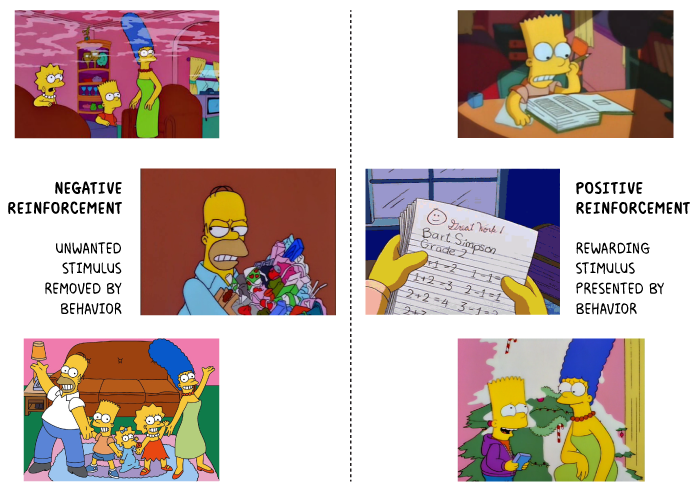
\includegraphics[width=200pt]{positive-negative-reinforcement.png}}
                        \caption{Reforço Positivo/Negativo}
                    \end{subfigure}
                    \begin{subfigure}[b]{.45\textwidth}
                        \centering
                        \raisebox{-0.5\height}{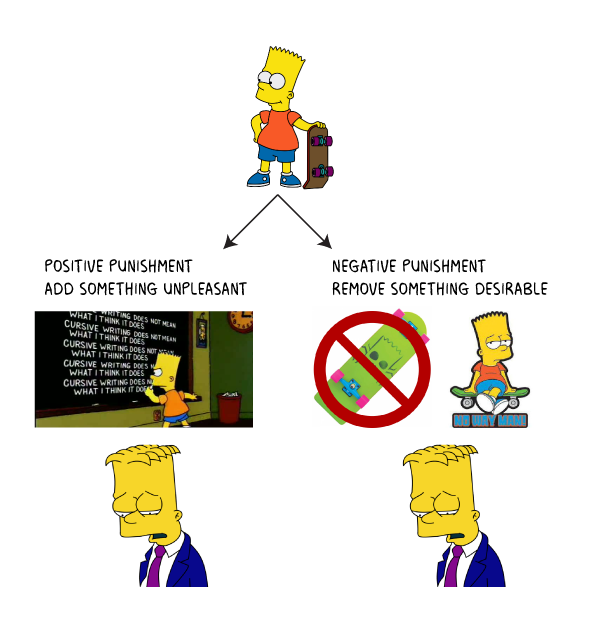
\includegraphics[width=180pt]{positive-negative-punishment_0.png}}
                        \caption{Punição Positiva/Negativa}
                    \end{subfigure}
                    \caption{Fonte: Shrestha (2017)}
                    \label{fig:reforco-punicao}
                \end{figure}
            
    \section{Exemplos}
    
        Um exemplo tradicional é o do cachorro que toca uma campainha, recebe um petisco e passa a tocar seguidamente para receber mais petiscos. Outro caso bastante conhecido, e muito utilizado pelos pais, é o da criança que pega na tomada, leva um choque e então aprende a não fazer isso novamente. Por fim, uma situação que vai nos ajudar bastante a ilustrar o Aprendizado por Reforço, e também muito utilizado em pesquisas, é a de um jogador aprendendo a jogar um jogo. De modo geral, os exemplos com jogos nos ajudam a rapidamente descrever o problema e visualizar a maneira como as técnicas de Aprendizado por Reforço os resolvem.
            
    \section{Características}
    
        \begin{itemize}
            \item Aprendizado através da interação com o ambiente;
            \item Caracterizado pelo aprendizado por tentativa e erro
            \item Recompensas futuras (delayed rewards);
            \item Problema de decisão sequencial
        \end{itemize}
        
        \subsection{Diferença de outros paradigmas}
        
            \todo{Além disso, o aprendizado por reforço é um terceiro paradigma de aprendizado diferente dos aprendizados supervisionado e não-supervisionado.\\
            No caso não-supervisionado, o objetivo é encontrar estruturas escondidas em coleções de dados.\\
            No caso supervisionado, o processo de aprendizado ocorre através de respostas instrutivas (instructive feedback), que indicam qual a resposta esperada.\\
            Já no RL, o aprendizado ocorre através de respostas avaliativas, que indicam um valor associado à ação.}
            
        \subsection{Tempo de resposta}
        
            Outra característica do Aprendizado por Reforço é a possível demora para receber uma resposta significativa. Por exemplo, em problemas de aprendizado por reforço a resposta é conhecida a cada iteração; já em problemas de otimização sabemos a distância para a função objetivo em todos os instantes. No caso do aprendizado por reforço temos tarefa de recompensas imediatas e tadias.
        
            \subsubsection{Recompensas imediatas}
        
                Em algumas tarefas, recompensas significativas são recebidas após cada iteração. Chamamos esse caso de \emph{recompensas imediatas}. Nesse caso, o agente poderá encontrar estratégias de curto prazo e ainda assim ser bem sucedido.
        
            \subsubsection{Recompensas tardia}
        
                Na maioria dos problemas o agente interage várias vezes com o ambiente antes de receber uma recompensa significativa. Por exemplo, em um jogo de xadrez cada jogador realizará dezenas de ações antes de saber a resposta final, vitória, derrota ou empate. Essa característica é chamada de \emph{recompensas tardias} (do inglês \emph{delayed rewards}). Para resolver esse tipo de problema é necessária a descoberta de estratégias de longo prazo.
        
    \section{Elementos}
    
        Nós temos uma entidade que é responsável pelo processo de entender o estado em que se encontra e executar uma ação. Essa entidade é o agente. 
    
        \begin{itemize}
            \item Ambiente;
            \item Modelo (opcional);
            \item Política;
            \item Função de valor;
            \item Recompensa.
        \end{itemize}
        
    \section{Diagrama de interação}
    
        \begin{center}
            \rlinteraction
        \end{center}
    
    \section{Breve história}
    
        Três correntes separadas.
        
        \subsection{Aprendizado por tentativa e erro (learning by trial)}
            Ideias iniciais de aprendizado por tentativa e erro na década de 1850;
            
            Discussão mais explícita a partir da década de 1890;
            
            Continua sendo desenvolvida pela psicologia no início do século XX;
            
            Primeiras implementações na década de 1950;
            
            Durante muito tempo, RL foi confundido com SL;
            
            Os termos “reforço” e “aprendizado por reforço” em problemas de tentativa e erro foram utilizados pela primeira vez na década de 1960.
    
        
        \subsection{Problemas de controle ótimo}
            Iniciado na década de 1950;
            
            Modelados como Processos de Decisão de Markov (MDP);
            
            Resolvidos através de técnicas de Programação Dinâmica.
    
        
        \subsection{Diferença temporal}
            Mais recente, fim dos anos 1980, com Watkins     (1989);
            
            Foi o que uniu as outras duas correntes, formando uma área só.
            
        \subsection{Marcos \emph{recentes} utilizando Aprendizado por Reforço}
        
            \begin{itemize}
                \item \textbf{2013}: Publicação no ArXiv do artigo seminal \emph{Playing Atari with Deep Reinforcement Learning} pela então \emph{DeepMind Technologies} \textcolor{red}{referenciar mnih 2013};
                \item \textbf{2015}: Publicação na revista \emph{Nature} do artigo \emph{Human-level control through deep reinforcement learning} pelo \emph{Google DeepMind}; \textcolor{red}{referenciar mnih 2015}
                \item \textbf{2017}: \emph{AlphaGo} vence Lee Sedol, campão mundial de Go;  \textcolor{red}{referenciar documentario alphago e o paper}
                \item \textbf{2019}: \emph{OpenAI Five} vence a equipe OG no jogo Dota2;  \textcolor{red}{referenciar openai five}
                \item \textbf{2019}: AlphaStar vence MaNa, jogador profissional de StarCraft II. \textcolor{red}{referenciar alphastar}
            \end{itemize}

    \section{Esperança}
            
        Ao longo dos estudos, um conhecimento básico em estatística seria muito útil. Mas certamente é essencial conhecer desde o início o conceito o de \emph{valor esperado} ou \emph{esperança}. Por sua importância e simplicidade, ele será apresentado agora.
        
        Considere uma variável aleatória $\RandomVariable{X}$ que pode assumir $k$ valores $x_1$, $x_2$, \dots, $x_k$. De acordo com uma distribuição de probabilidade $p$, cada um desses valores ocorre com uma probabilidade $p(x_1)$, $p(x_2)$, \dots, $p(x_k)$, respectivamente. A \emph{esperança} (ou \emph{valor esperado}) de $\RandomVariable{X}$ sob a distribuição $p$ é definida como:
        \begin{equation}
        \begin{aligned}
            \label{eq:state-value}
            \ExpectedValue_p[\RandomVariable{X}] & = \sum_i p(x_i) \cdot x_i \\
            & = p(x_1) \cdot x_1 + p(x_2) \cdot x_2 + \dots + p(x_k) \cdot x_k\ .
        \end{aligned}
        \end{equation}
        Na maioria dos casos, a distribuição de probabilidade $p$ é omitida, de modo que usamos a notação $\ExpectedValue[\RandomVariable{X}]$.

        Por exemplo, considere um dado de seis faces não viciado, $\RandomVariable{D}$. Ele pode assumir um dos valores $\{1, 2, 3, 4, 5, 6\}$, cada um deles com probabilidade $\frac{1}{6}$. Assim, o valor esperado de $\RandomVariable{D}$ é:
        \begin{equation*}
        \begin{aligned}
            \ExpectedValue[\RandomVariable{D}] & = \frac{1}{6} \cdot 1 + \frac{1}{6} \cdot 2 + \frac{1}{6} \cdot 3 + \frac{1}{6} \cdot 4 + \frac{1}{6} \cdot 5 + \frac{1}{6} \cdot 6 \\
            & = 3.5\ .
        \end{aligned}
        \end{equation*}        
        Note que o valor esperado é a média ponderada dos valores possíveis, em que a ponderação é dada de pela distribuição de probabilidade.
    
        \todo{O objetivo maior em tarefas de aprendizado por reforço é executar as ações cujas recompensas são máximas. Mais ainda, como há um conjunto de probabilidades envolvidas, desejamos executar as ações que deem a maior recompensa esperada. Para isso, utilizaremos bastante, entre outras coisas, o \emph{princípio da utilidade máxima esperada}.}

        O \emph{princípio da utilidade máxima esperada} diz que ... Ele foi desenvolvido por Von-Neumman e Morgenstern ...
        
        Formalmente, o teorema de Von-Neumman-Morgenstern nos diz que (equação) ... Podemos simplificar esse conceito da seguinte forma: considere que $x$ siga uma certa distribuição de probabilidade e para cada possibilidade $i$ teremos um valor $x_i$ associado, dizemos que o \emph{valor esperado} de $x$ é:
        \begin{equation}
            \mathbb{E} \left [ x \right ] = \sum_{i} p(i) \cdot x_i
        \end{equation}
        
        Por exemplo: (olhar o exemplo do caderno azul)
    
\end{document}